\section{ATM PERFORMANCE INDICATORS}
\label{sec:atm_indicators}

In the context of the performance-based management advocated by the International Civil Aviation Organization (ICAO), Key Performance Indicators (KPIs) are essential metrics used to quantitatively express past and current operational performance against organizational objectives. In the aviation industry, KPIs are crucial for enhancing governance and operational efficiency in a highly complex and regulated sector. By relying on standardized metrics, stakeholders can identify bottlenecks, measure outcomes, and promote continuous improvements in safety, punctuality, airport capacity, and environmental sustainability. 

Furthermore, the systematic analysis of KPIs facilitates communication among airport operators, airlines, air navigation service providers (ANSPs), and regulatory bodies, fostering a shared vision of strategic goals. KPIs also play a vital role in aligning aviation operations with international policies, such as the United Nations Sustainable Development Goals, by measuring environmental impacts like fuel consumption and emissions.

In this study, two specific performance indicators established by ICAO are of primary interest: KPI08: Additional Time in TMA, and KPI16: Additional Fuel Burn. Both metrics combined are essential to evaluate aircraft performance at Terminal Maneuvering Area (TMA) in terms of time, fuel consumption and emissions. However, this work focuses on the development of predictive models for KPI16, as predicting additional fuel burn is crucial for understanding and mitigating environmental impacts, as well as providing companies and air traffic managers actionable insights to optimize operations and reduce costs.

\subsection{KPI08: Additional Time in TMA}
KPI08 measures the additional transit time spent by an aircraft within the TMA compared to an unimpeded baseline, considered as the optimal transit time. In this study, the Terminal Area is defined as a cylindrical airspace with a 100-nautical-mile radius centered at Guarulhos (GRU) International Airport. The reference baseline is generally established through the clustering of transit time samples based on the runway in use, the aircraft type, and the entry sector into the terminal area. As illustrated in Figure \ref{fig:gru_sectors}, these entry sectors are divided into angular segments of 60 degrees. The unimpeded transit time is then defined as the 20th percentile of all samples within these grouped conditions. According to the MCA 100-22 methodology \cite{mca10022}, this 20th percentile threshold was established following ICAO recommendations, which identified that, statistically, the 20th percentile ($P_{20}$) provides a robust approximation of an unimpeded reference value. Additionally, this selection inherently incorporates a treatment for outliers in the operational dataset.

\begin{figure}[htbp]
    \centering
    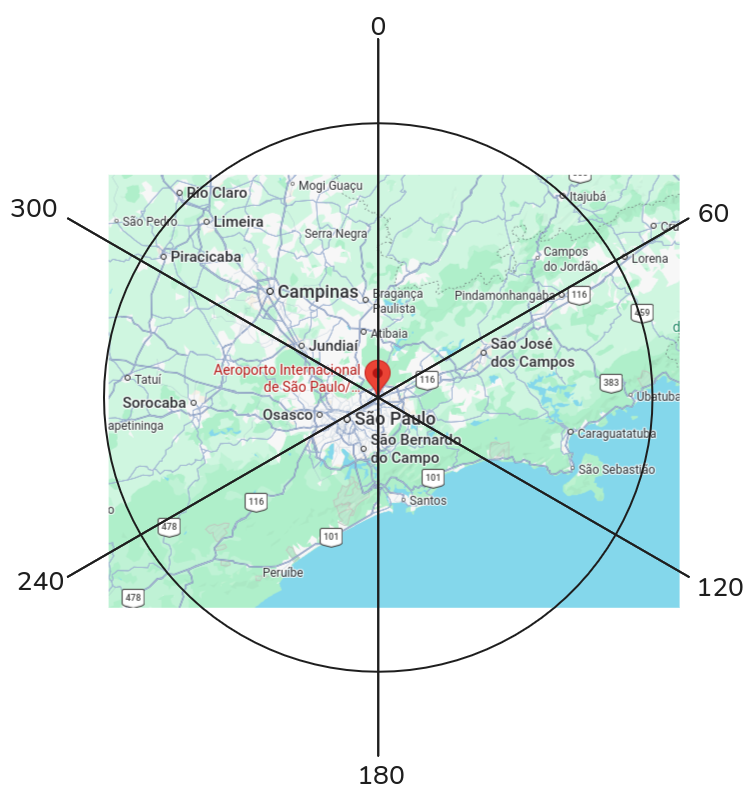
\includegraphics[width=0.8\linewidth]{images/gru_sectors.png}
    \caption{Guarulhos International Airport (GRU) Terminal Maneuvering Area (TMA) and its 60-degree entry sectors.}
    \label{fig:gru_sectors}
\end{figure}

Various factors can influence this indicator, including airspace design, meteorological conditions, and tactical interventions by Air Traffic Control (ATC) such as holding patterns and vectoring for sequencing. The comparison of the actual transit time to the 20th percentile baseline effectively isolates the operational inefficiencies, focusing on the ATM's responsibility in optimizing the arrival flow.

\subsection{KPI16: Additional Fuel Burn}
KPI16 represents the core metric for evaluating ATM-induced operational efficiency from an environmental perspective, providing an aggregate view of the excess fuel consumed during a flight phase. In the context of TMA operations, it is directly correlated with the inefficiencies captured by KPI08. 

There are various methods for calculating KPI16. In Brazil, the Department of Air Space Control (DECEA) adopts a strategy similar to KPI08, as the additional fuel burn is calculated as the difference between the actual fuel consumed by an aircraft and a reference fuel consumption. Like KPI08, this baseline is determined as the 20th percentile of fuel consumption for similar flights. Positive values of KPI16 indicate fuel consumption above the expected optimal level—often resulting from airspace congestion and ATC interventions—whereas negative values indicate flights that operated more efficiently than the established baseline. As the target variable of the predictive models developed in this work, KPI16 serves as a direct proxy for the environmental and economic cost of ATM inefficiencies in the terminal area.
